%%%%%%%%%%%%%%%%%%%%%%%%%%%%%%%%%%%%%%%%%%%%%%%%%%%%%%%%%%%%%%%%%%%%%%
% Overleaf (WriteLaTeX) Example: Molecular Chemistry Presentation
%
% Source: http://www.overleaf.com
%
% In these slides we show how Overleaf can be used with standard 
% chemistry packages to easily create professional presentations.
% 
% Feel free to distribute this example, but please keep the referral
% to overleaf.com
% 
%%%%%%%%%%%%%%%%%%%%%%%%%%%%%%%%%%%%%%%%%%%%%%%%%%%%%%%%%%%%%%%%%%%%%%

\documentclass{beamer}

\mode<presentation>
{
  \usetheme{Madrid}       % or try default, Darmstadt, Warsaw, ...
  \usecolortheme{default} % or try albatross, beaver, crane, ...
  \usefonttheme{default}    % or try default, structurebold, ...
  \setbeamertemplate{navigation symbols}{}
  \setbeamertemplate{caption}[numbered]
} 

\usepackage[english]{babel}
\usepackage[utf8x]{inputenc}
\usepackage{chemfig}
\usepackage[version=3]{mhchem}

\usepackage{hyperref}
  \hypersetup{colorlinks=true}
  \hypersetup{urlcolor=blue}
  \hypersetup{linkcolor = .}
\usepackage{xcolor}
\usepackage{siunitx}
  \sisetup{separate-uncertainty = true}
\usepackage{physics}
\usepackage[font=small,labelfont=bf]{caption}
\usepackage{subcaption}
\usepackage[en-GB]{datetime2}
\usepackage{overpic}
\usepackage{feynmp}
\DeclareGraphicsRule{*}{mps}{*}{}

\usepackage{scalerel}
\newcommand{\mylbrace}[2]{\vspace{#2pt}\hspace{6pt}\scaleleftright[\dimexpr5pt+#1\dimexpr0.06pt]{\lbrace}{\rule[\dimexpr2pt-#1\dimexpr0.5pt]{-4pt}{#1pt}}{.}}
\newcommand{\myrbrace}[2]{\vspace{#2pt}\scaleleftright[\dimexpr5pt+#1\dimexpr0.06pt]{.}{\rule[\dimexpr2pt-#1\dimexpr0.5pt]{-4pt}{#1pt}}{\rbrace}\hspace{6pt}}

% Here's where the presentation starts, with the info for the title slide
\title[University of Oxford]{BESIII Charm Meeting \\Measurement of CP even fraction $F_+$ in $D^0\to K^+K^-\pi^+\pi^-$}
\author{\textbf{Martin Tat} \hspace{0.54em} Guy Wilkinson \hspace{0.54em} Sneha Malde}
\institute{\normalsize University of Oxford \\ \vspace{0.3cm} \normalsize BESIII Charm Meeting \vspace{-0.3cm}}
\date{15th March 2022}

\titlegraphic{
\includegraphics[width = 2.0cm, height = 2.0cm]{OxfordLogo.pdf}\hspace{1cm}~%
              
\includegraphics[width = 3.2cm, height = 2.0cm]{bes3.jpg}}

\begin{document}

\begin{frame}
  \titlepage
\end{frame}

% These three lines create an automatically generated table of contents.
\begin{frame}{Outline}
  \tableofcontents
\end{frame}

\section{Introduction and motivation}
\begin{frame}{Introduction}
  \begin{itemize}
    \setlength\itemsep{0.5em}
    \item{Original plan (for my PhD):}
    \begin{itemize}
    \setlength\itemsep{0.2em}
      \item{$c_i$/$s_i$ analysis with new $\SI{20}{\per\femto\barn}$ BESIII $\psi(3770)$ dataset}
      \item{Develop binning scheme using LHCb model \href{https://arxiv.org/abs/1811.08304}{JHEP 02 (2019) 126}}
      \item{Perform model independent $\gamma$ measurement at LHCb simultaneously}
      \begin{itemize}
        \item{Expected precision $\Delta\gamma\approx 12^\circ$ with LHCb Run\,1+2}
      \end{itemize}
    \end{itemize}
  \end{itemize}
  \begin{figure}
    \centering
    \begin{subfigure}{0.5\textwidth}
      \centering
      \begin{overpic}[width=1.0\textwidth, clip=true, trim={10.0cm 2.7cm 0.8cm 0}]{Plots/d2kkpipi_fiveL_allDP.pdf}
        \put (55,58) {\scriptsize LHCb unofficial}
      \end{overpic}
      \caption{Fit of $B^\pm\to[K^+K^-\pi^+\pi^-]_D\pi^\pm$}
    \end{subfigure}%
    \begin{subfigure}{0.5\textwidth}
      \centering
      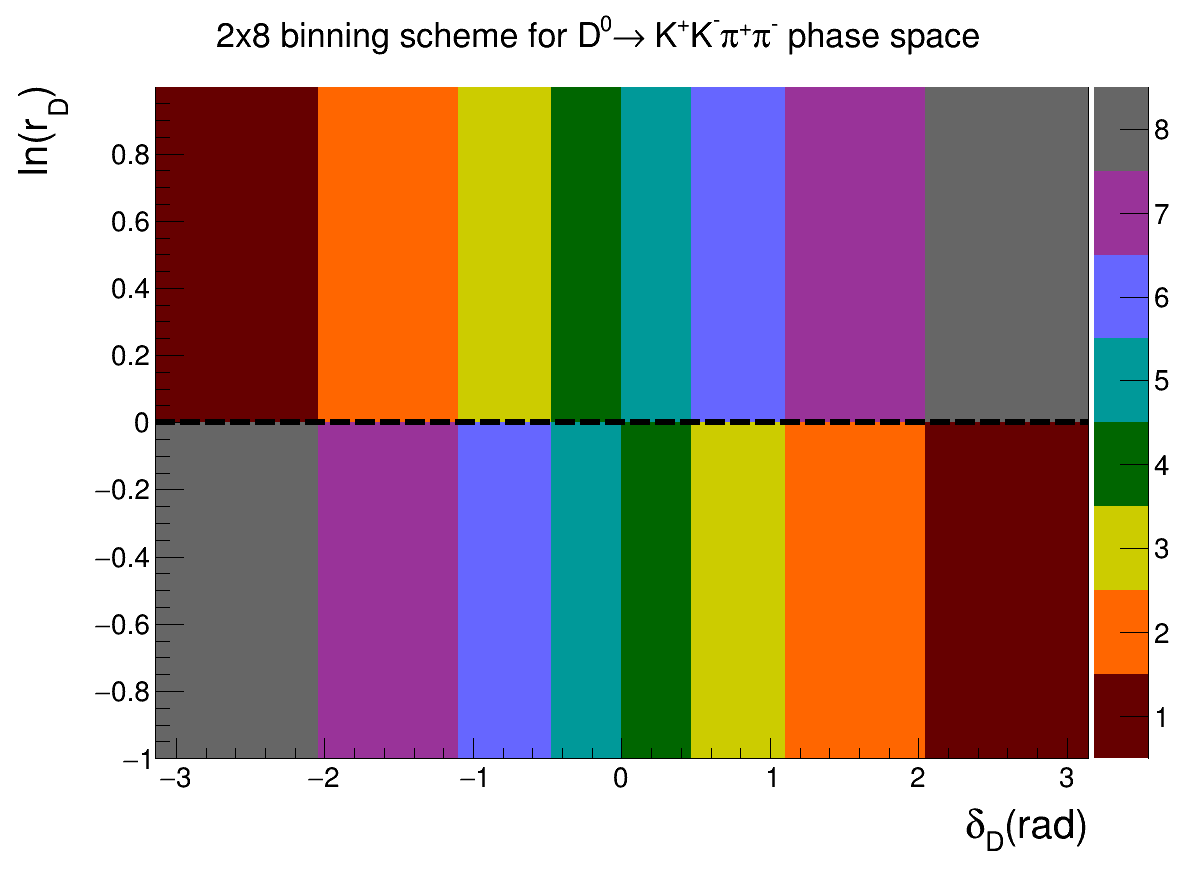
\includegraphics[width=\textwidth]{Plots/BinningSchemePlot_8Bins.png}
      \caption{Binning scheme for $D^0\to K^+K^-\pi^+\pi^-$}
    \end{subfigure}
  \end{figure}
\end{frame}

\begin{frame}{Motivation}
  \begin{itemize}
    \setlength\itemsep{1.5em}
    \item{CP even fraction $F_+$ describes the CP content of a self-conjugate multi-body decay}
    \begin{itemize}
      \item{$F_+ = 1$ ($0$) for CP even (odd) final states}
    \end{itemize}
    \item{$F_+$ can be measured with current $\SI{3}{\per\femto\barn}$ dataset}
    \begin{itemize}
      \item{Useful cross check of LHCb amplitude model}
      \item{Allows current analyses to include $KK\pi\pi$ as a GLW mode}
    \end{itemize}
    \item{Important input to quasi-GLW analysis of the CKM angle $\gamma$}
    \begin{itemize}
      \item{Current GLW modes: $KK$, $\pi\pi$, $\pi\pi\pi\pi$}
      \item{Small effort to include $KK\pi\pi$ to gain more statistics!}
    \end{itemize}
    \item{Other $F_+$ measurements:}
    \begin{itemize}
      \item{$D^0\to\pi^-\pi^-\pi^+\pi^-$ \href{https://arxiv.org/abs/1709.03467}{JHEP 01 (2018) 144}}
      \item{$D^0\to K_S\pi^+\pi^-\pi^0$ \href{https://arxiv.org/abs/1710.10086}{JHEP 01 (2018) 82}}
      \item{Both measurements are from CLEO-c, BESIII analyses ongoing}
    \end{itemize}
  \end{itemize}
\end{frame}

\section{Theory of strong phase analysis}
\begin{frame}{Strategy for $c_i$/$s_i$ analysis}
\end{frame}

\section{Selection and tag modes}
\begin{frame}{Selection}
  \begin{figure}
    \centering
    \includegraphics[width=\textwidth]{example-image-a}
  \end{figure}
\end{frame}

\begin{frame}{Tag modes}
  \begin{figure}
    \centering
    \begin{subfigure}{0.5\textwidth}
      \centering
      \includegraphics[width=\textwidth]{example-image-a}
    \end{subfigure}%
    \begin{subfigure}{0.5\textwidth}
      \centering
      \includegraphics[width=\textwidth]{example-image-a}
    \end{subfigure}
  \end{figure}
\end{frame}

\section{Determination of single and double tag yields}

\section{Initial look at \texorpdfstring{$K_i$}{Ki}}

\section{\texorpdfstring{$F_+$}{F+} measurement with CP tags}

\section{\texorpdfstring{$F_+$}{F+} measurement with \texorpdfstring{$K_{S, L}\pi^+\pi^-$}{KSpipi} tags}

\section{Summary and conclusion}

\begin{frame}{Summary}
  \begin{center}
    {\huge Thank you!}
  \end{center}
\end{frame}
    

\end{document}
